\documentclass[12 pt]{article}
\usepackage{hyperref, fancyhdr, setspace, enumerate, amsmath,
  lastpage, amssymb}
\usepackage[margin=1 in]{geometry}
\allowdisplaybreaks
%\usepackage[dvipsnames]{xcolor}   %May be necessary if you want to color links
\hypersetup{
	%colorlinks=true, %set true if you want colored links
	linktoc=all,     %set to all if you want both sections and subsections linked
	linkcolor=black,  %choose some color if you want links to stand out
}
\usepackage{graphicx}
\graphicspath{{Images/}}
\author{Julian Lore}
\date{Last updated: \today}
\title{MATH 324: Statistics}
\pagestyle{fancy}
\lhead{MATH 324}
\chead{\leftmark}
\rhead{Julian Lore}
\cfoot{Page \thepage \ of \pageref{LastPage}}
\newcommand{\tab}[1]{\hspace{.2\textwidth}\rlap{#1}}
\begin{document}
	\onehalfspacing
	\maketitle
	Notes from Masoud Asgharian's Winter 2018 lectures.
	\tableofcontents
        \section{01/09/18}
        \paragraph{What we will cover this semester}
        Will essentially cover chapter 8,9,10. For chapter 11, he will
        give us his own notes. The first 6 sections of chapter 13 and
        a few sections from chapter 14. Occasionally we will go back
        to chapter 7 to revisit things like the t distribution.
        \\ In 323, we made probabilistic models. Statistics is the
        breach in which we connect these models to real
        life. Otherwise, those are just models. A core part of data
        analysis and data sciences is statistics and computer
        science.
        \subsection{Overview - What is Statistics?}
        Inductive logic, we have a sample from the population we want
        to make inference about. With this data, we want to extend the
        results to the whole population. From small to large, sample
        to the population.
        % Image
        \\ 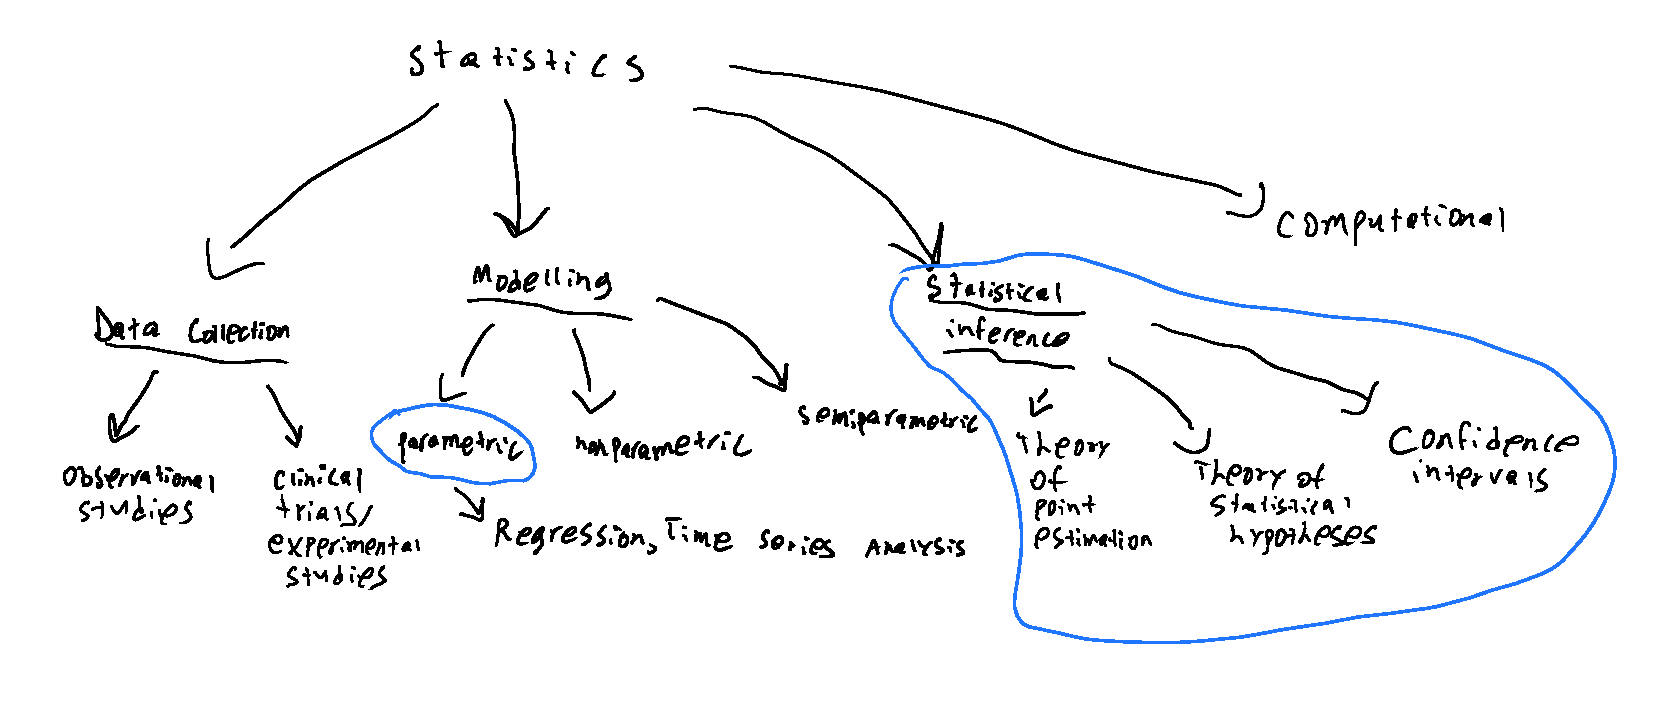
\includegraphics[width=\textwidth]{i1.pdf}
        \begin{itemize}
        \item Observational studies: we go to the population and make
          observations.
        \item Experimental studies: give test subjects something,
          i.e. give them cigarettes when trying to test for if
          cigarettes lead to cancer. Need
          to account for causation, other factors that can affect
          outcome. In order to do so we have to keep their diet and
          other factors controlled. We must also have some sort of
          randomization, we can't send all males to one group and all
          females to another, as males may have a tendency to smoke or
          something of the like. These are also called clinical
          trials.
        \item When we have data, the next step is modeling. May
          occasionally speak of this, but this is not part of the
          course. There are different approaches to modeling, can be
          split into 3 parts.
          \begin{itemize}
          \item Parametric: the salary is distributed like a
            distribution (ex. Gamma), but we don't know the
            parameters. Take for example, we always know that the
            normal distribution is a bell curve, but we don't know
            where it's centered. Very useful, but we might have a
            miss-specification. How do we know our models are correct?
            Most of the time we will be talking about
            \textbf{parametric} models.
          \item Semiparametric
          \item Nonparametric: since we don't know if parametric
            models are correct, we make no assumption about the
            distribution. We just assume that $X \sim F$, all we
            assume about $F$ is that it's continuous, nothing
            more. This is an infinite dimensional vector. Why? How do
            we know a function? We have a vector for $F$, like
            $F(1),F(2, \ldots)$. How do we approximate this? $X_i
            \stackrel{iid}{\sim}F, i=1,2,\ldots,n$. $n$ patients, with
            all the same distribution. So $F(t)=P(X\leq t)$. What does
            this tell us? The proportion of time that $x$ falls below
            $t$. So with $n$ samples, how do we mimic this? We count
            the number of observations below $t$, i.e. $\frac{\#X_i
              \leq t}{n}$, which is an approximation of the
            above. This is an empirical observation. More
            mathematically:
            \begin{equation*}
              \varepsilon(t) =
              \begin{cases}
                1 & \text{if }t\geq 0
                \\ 0 & \text{otherwise}
              \end{cases}
            \end{equation*}
          So we have
          $\hat{F}_n(t)=\frac{1}{n}\sum_{i=1}^n\varepsilon(t-x_i)$. This
          gives us a binomial distribution. But we are assuming they
          are all the same distribution.
          \\ Nonparametric approaches are good for functions of single
          variables, but not for multi variables, which is what
          semiparametric was made for.
          \end{itemize}
          \item Bayesian inference: when you learn that $X \sim N(\mu,
            \sigma^2)$, $X$ is normally distributed and $\mu$ is the
            average of the whole population. Bayes' approach says that
            these parameters are not constants, these are random
            variables themselves. Bayes did not look at probability as
            a frequentest approach, not the proportion of when something
            arrives (frequentest approach works when we have a huge
            sample). The other approach that Bayes had was an updating
            approach, that our parameters are unknown. This is good
            for when you have a stream of data (machine learning is a
            prime example). We have a lack of knowledge and then we
            update it using Bayesian's approach. $\to X | \mu,
            \sigma^2 \sim N (\mu, \sigma^2)$, i.e. the parameters are
            also normally distributed.
          \end{itemize}
          Most of the time we'll be at parametric modeling and
          statistical inference.
        \subsection{Point Estimation} What do we mean by point
        estimation? A scientific guess about the unknown parameter of
        the population. Consider the following situation:
        \\ $x_1, \ldots, x_n \sim N(\mu, 1)$ (usually interested in
        the normal distribution, binomial and poisson). Suppose this
        is the IQ of high school graduates in Canada (the $x_i$ are
        numbers). Why do we call this distribution normal? Because for
        a healthy population, most of the weight should be in the
        middle, just like the bell curve. The Normal distribution is
        especially important for modeling error. For insurance
        companies, we see at the tails that there aren't many large
        claims.
        \\ We want to find $\mu$. Recall that $E(X_i)=\mu,
        i=1,2,\ldots,n$ (if they all have the same observations, they
        have the same mean).
        \\ First, what is a point estimation? What properties should
        it have? If we know the value of $\mu$, we have the whole
        thing, can calculate everything. How do we estimate this? The
        whole population is huge, so we take a sample part of the
        population, mimicking the real $\mu$, getting $\overline{X}_n
        = \frac{1}{n}\sum_{i=1}^nX_i$. $\overline{X}_n$ is useful, but
        $\overline{X}_n-\mu$ isn't, as there's an unknown we have
        here.
        \paragraph{Statistic} A function of observations that does not
        depend on any unknown parameter.
        \subparagraph{Ex} $\overline{X}_n$ is a
        statistic. $\overline{X}_n - \mu$ is not.
        \paragraph{Estimator} A statistic that aims at estimating an
        unknown parameter (we want to work with it). For example, if
        $\mu$ moves from $-\infty$ to $\infty$, we want to have an
        estimator that also has the same range, not one that is
        strictly positive. Example: $\overline{X}_n$ is an
        estimator. However, consider:
        $$S^2 = \frac{1}{n-1}\sum_{i=1}^n(X_i-\overline{X}_n)^2$$
        This is a statistic, but not an estimator, it always returns a
        positive value. Also, take for example in physics, where each
        measure has a unit of measurement. This statistic wouldn't
        even be the same unit, so it once again is a bad estimator.
        \\ When we take a mean and try to estimate it, the next step
        is to figure out how we quantify possible bias.
        \\ \rule{\textwidth}{0.5 pt}
        $$\varepsilon = |\overline{X}_n-\mu |$$
        We can use Tchbyshev's inequality to put a bound on the
        error.
        \begin{flalign*}
        P(|X-\underbrace{E(X)}_{\mu_x}|>k\sqrt{\underbrace{Var(X)}_{\sigma_x^2}})
        \\ P(|X-\mu_x>k\sigma_x) \leq \frac{1}{k^2}
        \end{flalign*}
        Very useful, assume very little but get lots of
        information. One of the big hammers of probability and
        statistics. The only thing we assume here is the existence of
        the second moment.\\
        Consider $k=3$.
        \begin{flalign*}
          P(|X-\mu_x|>3\sigma_x)\leq \frac{1}{9}
          \\ P(|X-\mu_x|\leq 3 \sigma_x)\geq 1 - \frac{1}{9}\approx \%89
        \end{flalign*}
        Without knowing anything else about the distribution, this
        tells us that about $89\%$ of the population is within $3$
        times the variance of the mean.
\end{document}